\chapter{Access Control}

Il controllo degli accessi è un elemento centrale nella sicurezza informatica ed è definito da varie organizzazioni (ITU-T, NIST, \dots).

Il controllo degli accessi implementa una politica di sicurezza che specifica chi o
cosa (ad es un processo) può avere accesso a ciascuna specifica risorsa di sistema
e il tipo di accesso consentito in ogni caso

\subsubsection{Principi del AC}
\begin{itemize}
    \item \textbf{Autenticazione}: verifica validità delle credenziali.
    \item \textbf{Autorizzazione}: concessione dei permessi/diritti per accedere a una risorsa.
    \item \textbf{Auditing}: revisione e verifica indipendente delle attività.
\end{itemize}

\subsubsection{Elementi del AC}
\begin{itemize}
    \item \textbf{Soggetto}: l'entità che accede alle risorse, come un utente o un processo.
    \item \textbf{Oggetto}: la risorsa protetta, che può essere un file, una directory o un programma.
    \item \textbf{Diritti di accesso}: definiscono le operazioni che il soggetto può eseguire sull'oggetto.
\end{itemize}

\section{Politiche di Controllo degli Accessi}

\subsection{DAC (Controllo Discrezionale degli Accessi)}
Il DAC controlla l'accesso sulla base dell'identità del entità richiedente e delle regole definite (auth).

Viene definito \textit{discrezionale} perché un’entità potrebbe avere i
privilegi di accesso che le permettono, a sua
discrezione, di concedere, a un’altra entità,
l’accesso a una determinata risorsa.

Spesso viene fornito utilizzando una matrice di accesso:
\begin{itemize}
    \item elenca i soggetti in una dimensione (righe)
    \item elenca gli oggetti nell'altra dimensione (colonne)
\end{itemize}
La matrice spesso è sparsa.

\begin{figure}[ht]
    \centering
    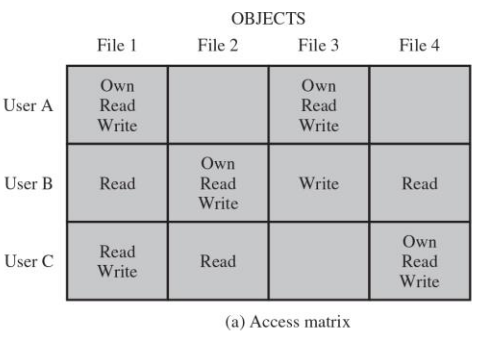
\includegraphics[width=0.6\linewidth]{chapters/images2/dac.png}
    \caption{Matrice DAC}
\end{figure}


\subsection{MAC (Controllo Obbligatorio degli Accessi)}
Il MAC utilizza etichette e autorizzazioni di sicurezza per garantire che solo utenti con i giusti privilegi possano accedere a determinate risorse, è uno dei sistemi più sicuri.

Questa politica è definita obbligatoria perché è
un'entità che ha l'autorizzazione accedere a una
risorsa non può, solo di sua spontanea volontà,
consentire a un'altra entità di farlo accedere a
quella risorsa.

\subsubsection{Vantaggi}
\begin{itemize}
    \item \textbf{Sicurezza Elevata:} a prova di manomissione; politiche di accesso non alterabili dagli utenti.
    \item \textbf{Automazione:} completa automatizzazione, riduzione del rischio di errori umani.
    \item \textbf{Integrità dei Dati:} i dati non possono essere modificati senza autorizzazione.
\end{itemize}

\subsubsection{Svantaggi}
\begin{itemize}
    \item \textbf{Pianificazione Complessa:} progettazione iniziale che può richiedere tempo e risorse elevate.
    \item \textbf{Manutenzione e Aggiornamenti:} controlli e aggiornamenti regolari dei diritti di accesso.
    \item \textbf{Risorse Amministrative:} spesso solo admin è autorizzato a gestire i diritti di accesso.
\end{itemize}

\subsection{RBAC (Controllo degli Accessi Basato su Ruoli)}
L'accesso alle risorse è regolato in base ai ruoli degli utenti all'interno del sistema. 
Viene utilizzato nei sistemi organizzativi. 

Ci sono quattro tipi di entità:
\begin{itemize}
    \item \textbf{Utente:} una persona che ha accesso al sistema informatico; ogni individuo ha un ID associato
    \item \textbf{Ruolo:} una funzione lavorativa all'interno dell'organizzazione che controlla il sistema
    \item \textbf{Autorizzazione:} approvazione di una particolare modalità di accesso a uno o
    più oggetti
    \item \textbf{Sessione:} una mappatura tra un utente e un sottoinsieme attivato
    dell'insieme di ruoli a cui è assegnato l'utente
\end{itemize}

\subsection{ABAC (Controllo degli Accessi Basato su Attributi)}
ABAC controlla l'accesso basandosi su attributi dell'utente e condizioni ambientali.

\section{Domini di Protezione}
I domini di protezione rappresentano un insieme di oggetti con i rispettivi diritti di accesso per ciascuno di essi. Ogni utente ha un proprio dominio, e i processi generati da tale utente ereditano i suoi permessi. L'associazione tra un processo e un dominio può essere statica o dinamica:
\begin{itemize}
    \item \textbf{User Mode}: alcune aree della memoria sono protette e certe istruzioni non sono eseguibili.
    \item \textbf{Kernel Mode}: è possibile eseguire istruzioni privilegiate e accedere a memoria protetta.
\end{itemize}
Il soggetto utilizza i diritti di accesso per interagire con l'oggetto in base alle politiche di sicurezza.

\section{Access Control in Sistemi Operativi}

\subsection{UNIX Security Model}
UNIX usa un modello di controllo degli accessi tramite utenti, gruppi e permessi su file. 

Gli ID degli utenti (UID) e i gruppi (GID) giocano un ruolo chiave. L'utente root (UID = 0) ha accesso a tutto.

\subsection{Windows Security Architecture}
Windows ha un'architettura di sicurezza complessa costituita principalmente da:
\begin{itemize}
    \item ACL (Access Control Lists) e SID (Security Identifiers)
    \item Sistema SRM (Security Reference Monitor): esegue controlli di accesso in modalità kernel
    \item Ogni processo ha un set di tokens chiamato \textit{security context} che ne definisce i permessi.
\end{itemize}

\begin{figure}[ht]
    \centering
    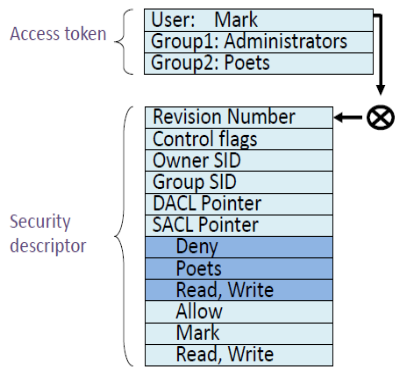
\includegraphics[width=0.5\linewidth]{chapters/images2/security-descriptor.png}
\end{figure}

Ogni oggetto ha un \textit{security descriptor} che contiene:
\begin{itemize}
    \item possessore e gruppo primario dell'oggetto
    \item diritti di accesso per gli utenti e i gruppi+
\end{itemize}

Quando un processo vuole accedere a un file oggetto, presenta il suo insieme di token (security context);
Windows controlla se il security context ha accesso all'oggetto basato sul descrittore di sicurezza dell'oggetto.


\section{Elementi di Sicurezza Specifici}

\subsection{SetUID e SetGID in UNIX}
Ogni processo in un sistema ha tre diversi ID utente:
\begin{itemize}
    \item \textbf{Effective User ID (EUID)}: determina le autorizzazioni del processo.
    \item \textbf{Real User ID (RUID)}: identifica l'utente che ha avviato il processo.
    \item \textbf{Saved User ID (SUID)}: memorizza l'EUID prima di eventuali modifiche.
\end{itemize}

\noindent Inizialmente, questi tre ID hanno lo stesso valore, corrispondente all'utente che ha avviato il processo.
SetUID e SetGID permettono temporaneamente di eseguire con i privilegi del proprietario di un file.

\subsection{MAC in Windows}
Windows utilizza un sistema di controllo MAC con diversi livelli di integrità che impediscono l'accesso non autorizzato.
Microsoft ha implementato livelli di integrità tramite i SID.

